\documentclass{article}


\usepackage{arxiv}
\usepackage{float}
\usepackage[utf8]{inputenc} % allow utf-8 input
\usepackage[T1]{fontenc}    % use 8-bit T1 fonts
\usepackage{hyperref}       % hyperlinks
\usepackage{url}            % simple URL typesetting
\usepackage{booktabs}       % professional-quality tables
\usepackage{amsfonts}       % blackboard math symbols
\usepackage{nicefrac}       % compact symbols for 1/2, etc.
\usepackage{microtype}      % microtypography
\usepackage{lipsum}
\usepackage{graphicx}
\usepackage{caption}
\usepackage{subcaption}
\usepackage[compact]{titlesec}
\titlespacing{\section}{0pt}{*0}{*0}
\titlespacing{\subsection}{0pt}{*0}{*0}
\titlespacing{\subsubsection}{0pt}{*0}{*0}


\title{Learning priors for adversarial autoencoders}

\author{
Belozerova Polina\\
Skoltech\\
\texttt{bel.pol.4@gmail.com} \\
%% examples of more authors
\And
Safin Alexander \\
Skoltech\\
\texttt{safinsam@yandex.ru} \\
\And
Pavlovskaia Natalia \\
Skoltech\\
\texttt{ya-ne-bo@yandex.ru} \\
}

\begin{document}
    \maketitle

    \begin{abstract}
        Most deep latent factor models choose simple priors for simplicity, tractability or
        not knowing what prior to use. Recent studies show that the choice of the prior
        may have a profound effect on the expressiveness of the model, especially when
        its generative network has limited capacity. In this paper, we propose to learn a
        proper prior from data for adversarial autoencoders (AAEs). We introduce the
        notion of code generators to transform manually selected simple priors into ones
        that can better characterize the data distribution. Experimental results show that
        the proposed model can generate better image quality and learn better disentangled
        representations than AAEs in both supervised and unsupervised settings. Lastly,
        we present its ability to do cross-domain translation in a text-to-image synthesis
        task.

        We took here several attempts to create a generative model. The main source of inspiration is \cite{original}.
        The results are presented for MNIST and CIFAR-10 datasets.
        We haven't achieve the same quality as in the original paper, but learnt a lot.
    \end{abstract}

    \section{Introduction}

    \subsection{Goal}
    Our goal is to reproduce the "Learning priors for adversarial autoencoders" \cite{original}

    \section{Algorithms}
    \subsection{Adversarial Autoencoder}
    Our baseline model is "Adversarial Autoencoders" \cite{DBLP:journals/corr/MakhzaniSJG15}
    \begin{center}
        \begin{figure}[H]
            \centering
            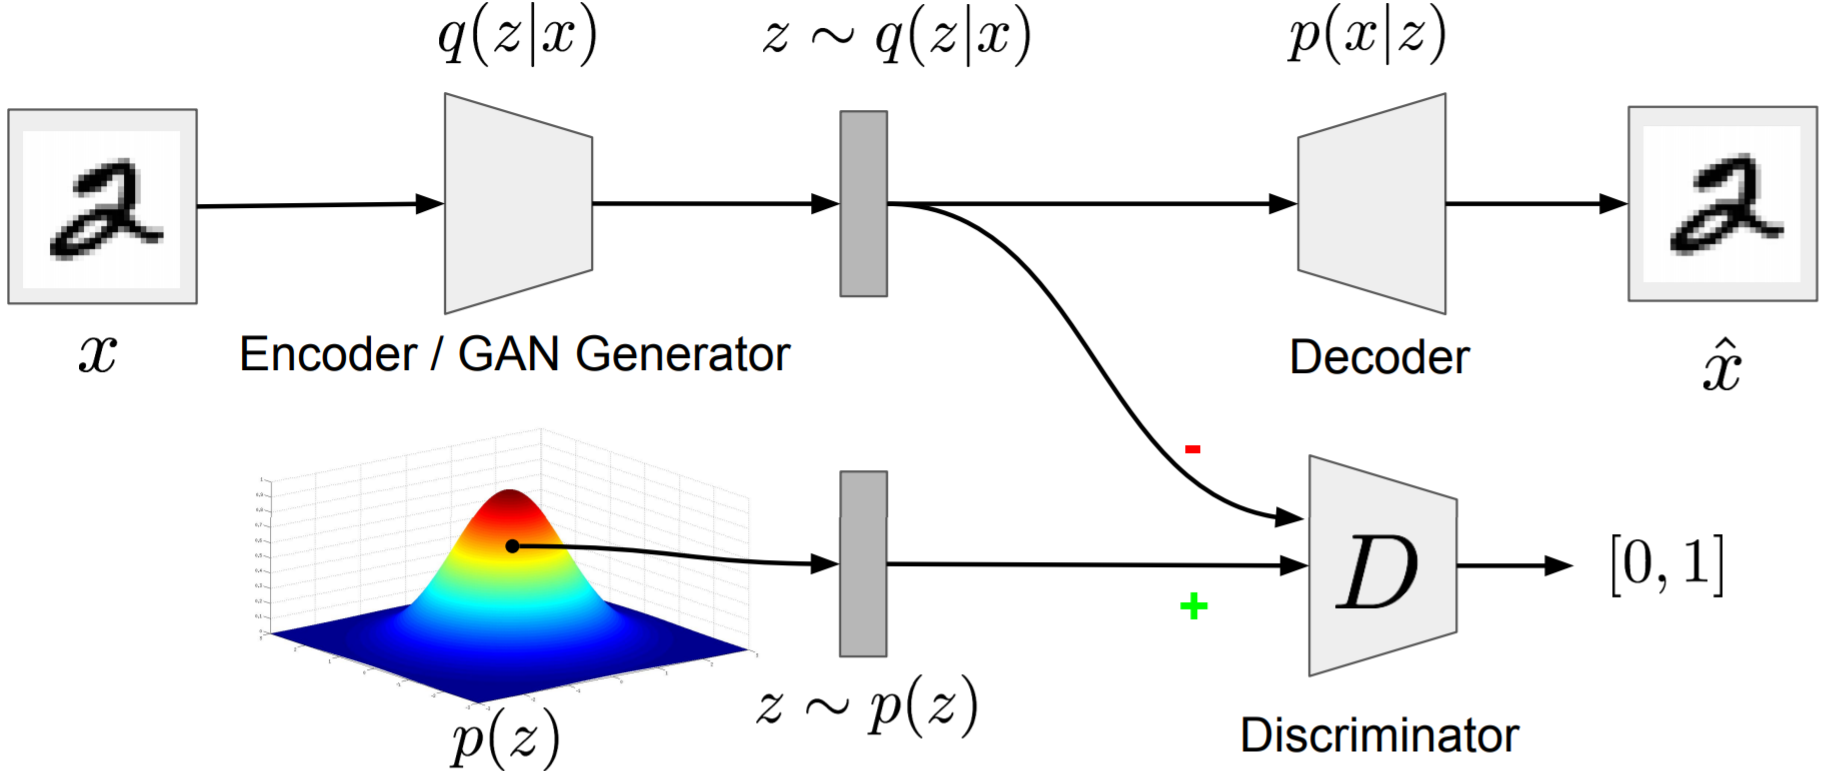
\includegraphics[width=0.25\textwidth]{figures/aae.png}
            \caption{Adversarial Autoencoder scheme}
        \end{figure}
    \end{center}
    \subsection{Original paper algorithm}
    \begin{center}
        \begin{figure}[H]{\textwidth}
            \begin{subfigure}{0.5\textwidth}
                \centering
                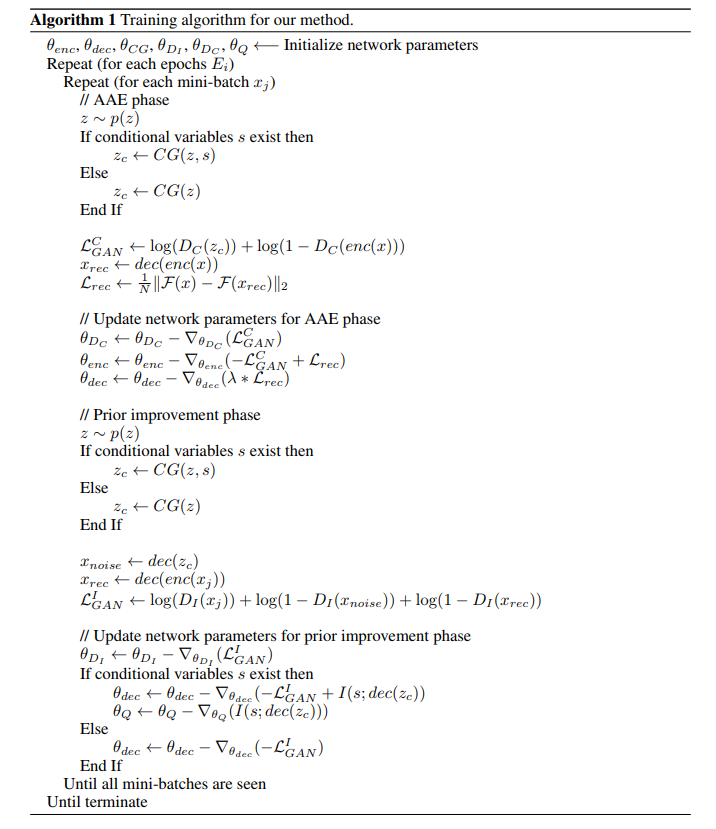
\includegraphics[width=0.75\linewidth]{figures/original-code.png}
                \caption{Original paper algorithm pseudo code}
            \end{subfigure}
            \begin{subfigure}{0.5\textwidth}
                \centering
                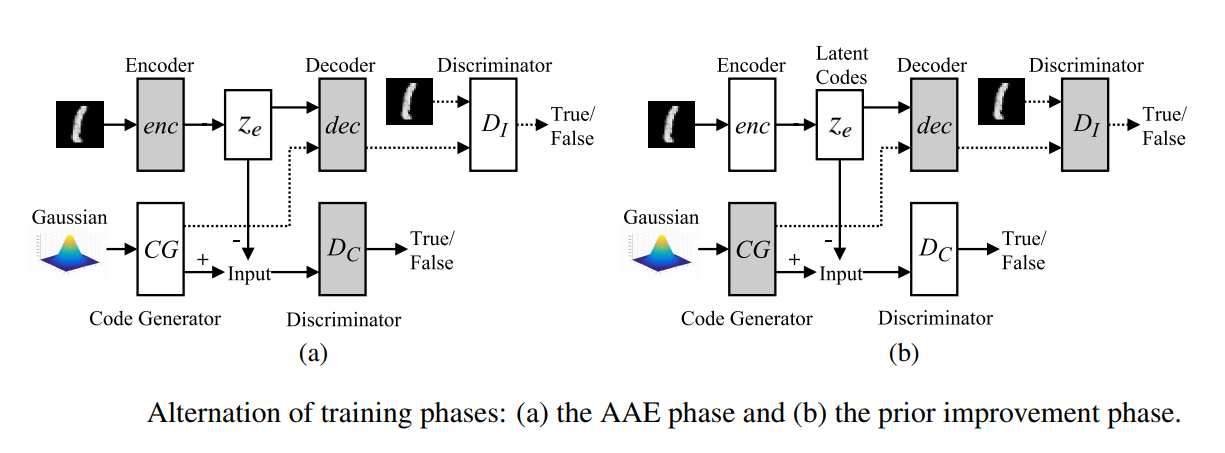
\includegraphics[width=0.75\linewidth]{figures/original.png}
                \caption{Original paper algorithm scheme}
            \end{subfigure}%
            \caption{Original paper algorithm}
        \end{figure}
    \end{center}

    \subsection{Additional algorithm}
    Is inspired by "Autoencoding beyond pixels using a learned similarity metric"\cite{DBLP:journals/corr/LarsenSW15}
    \begin{center}
        \begin{figure}[H]{\textwidth}
            \begin{subfigure}{0.5\textwidth}
                \centering
                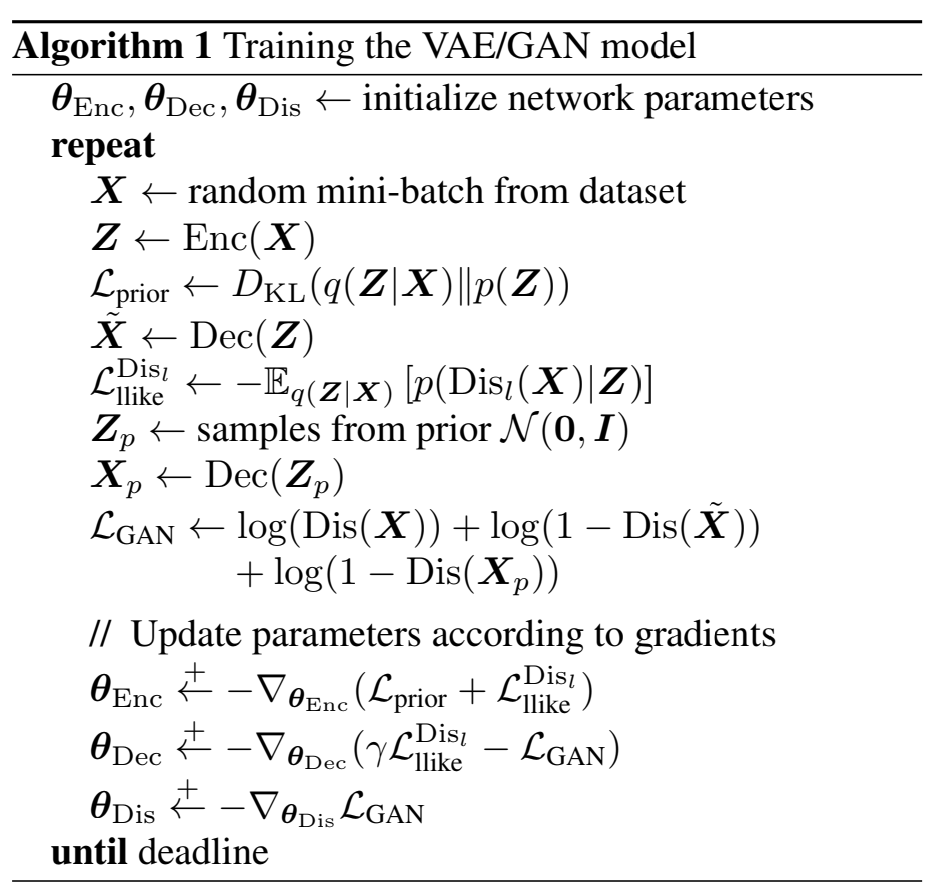
\includegraphics[width=0.5\linewidth]{figures/additional-code.png}
                \caption{Additional paper algorithm pseudo code}
            \end{subfigure}
            \begin{subfigure}{0.5\textwidth}
                \centering
                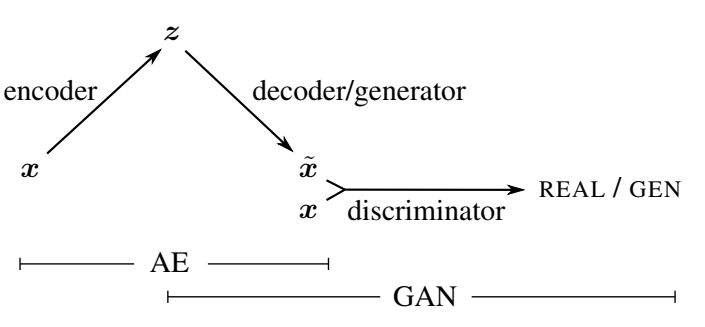
\includegraphics[width=0.5\linewidth]{figures/additional.png}
                \caption{Additional paper algorithm scheme}
            \end{subfigure}%
            \caption{Additional paper algorithm}
        \end{figure}
    \end{center}


    \section{Data}
    We made experiments for MNIST and CIFAR-10 datasets.

    \section{Problems and solutions}
    Problems
    \begin{itemize}
        \item Different formulae in the text and the pseudo code in the original paper
        \item 1 epoch even for MNIST takes about 17 minutes
        \item We had no time to try supervised setting
    \end{itemize}
    Solutions
    \begin{itemize}
        \item Using other papers and do updates according to the our own understanding
        \item Several updates of encoder-decoder
        \item Adjusting learning rates
    \end{itemize}
    \section{Results}
    \subsection{Results for AAE, Alexander}
    \begin{center}
        \begin{figure}[H]
            \centering
            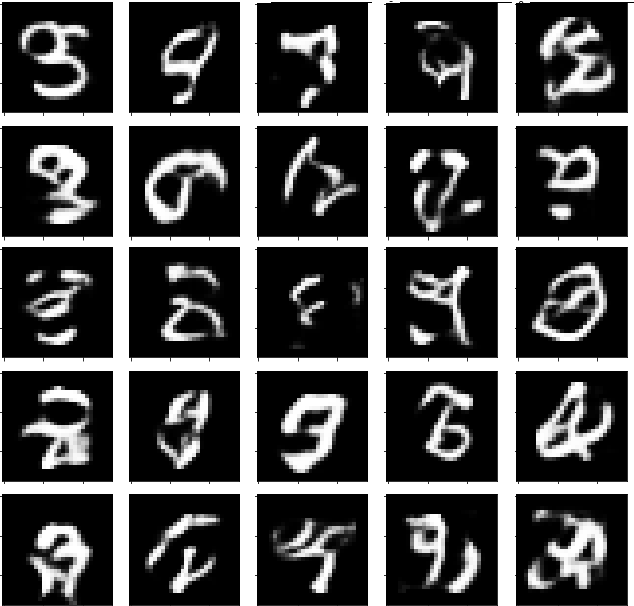
\includegraphics[width=0.2\textwidth]{figures/aae_epoch100.png}
            \caption{Samples from AAE on MNIST}
        \end{figure}
    \end{center}
    \subsection{Results for original paper}
    \subsection{Alexander's results}
    Training approach
    \begin{itemize}
        \item AAE-phase:\\
        \begin{itemize}
            \item Encoder update: $-\log(D_{code}(fake)+\varepsilon)) + L2$
            \item Code disc update (every 5 steps): \\ $-\left(\log(D_{code}(real)+\varepsilon) + \log(1 - D_{code}(fake)+\varepsilon)\right)$
            \item Decoder update: $L2$
        \end{itemize}\\
        \item Prior improvement phase (once in epoch):\\
        \begin{itemize}
            \item Decoder update: $-\log(D_{code}(sampled)+\varepsilon))$
            \item Code gen update: $-\log(D_{code}(sampled)+\varepsilon))$
            \item Image disc update:
            \begin{equation*}
                \begin{split}
                    &-(\log(D_{code}(real)+\varepsilon) + \log(1 - D_{code}(fake)+\varepsilon) + \\
                    &+ \log(1 - D_{code}(sampled)+\varepsilon) ) \\
                \end{split}
            \end{equation*}
        \end{itemize}
    \end{itemize}
    \begin{center}
        \begin{figure}[H]{\textwidth}
            \begin{subfigure}{0.5\textwidth}
                \centering
                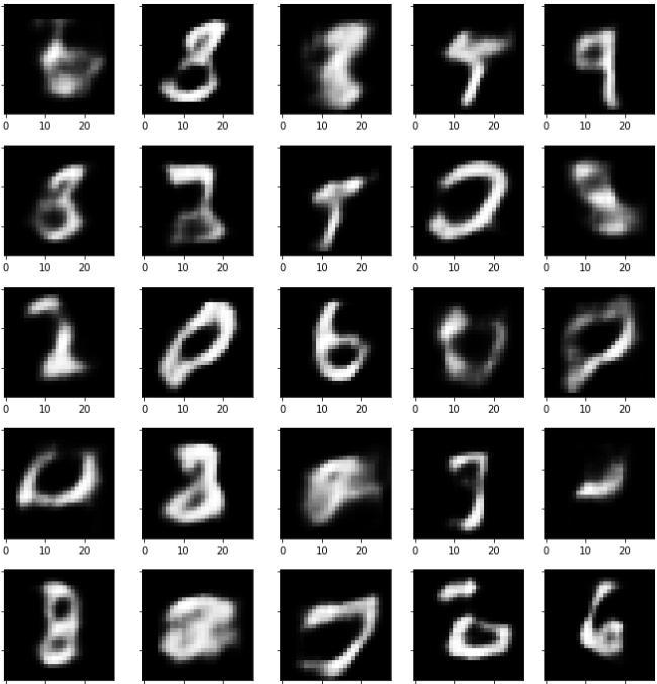
\includegraphics[width=0.35\linewidth]{figures/epoch8.png}
                \caption{MNIST, 8 epochs}
            \end{subfigure}
            \begin{subfigure}{0.5\textwidth}
                \centering
                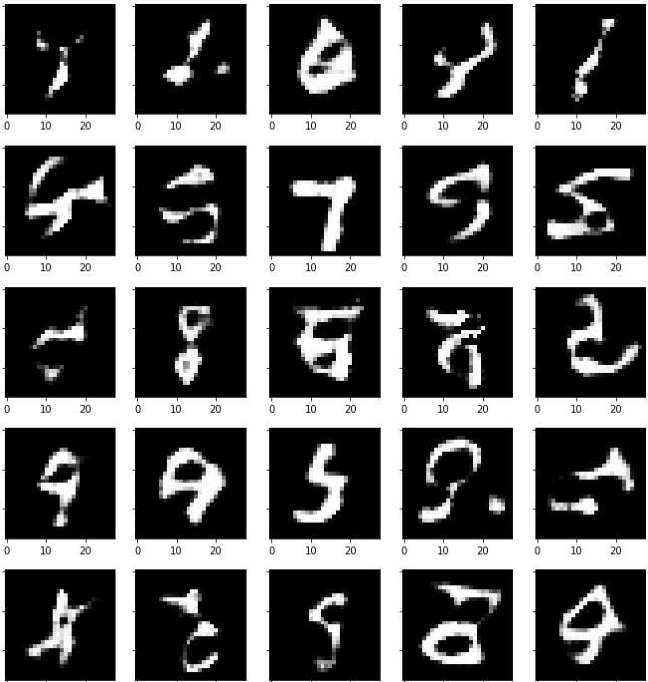
\includegraphics[width=0.35\linewidth]{figures/epoch100.png}
                \caption{MNIST, 100 epochs}
            \end{subfigure}%
            \caption{Original paper algorithm results for different epochs}
        \end{figure}
    \end{center}

    \begin{center}
        \begin{figure}[H]
            \centering
            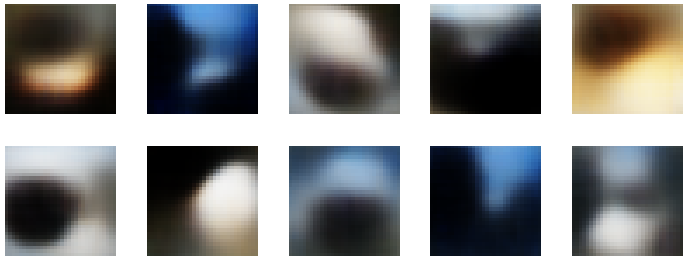
\includegraphics[width=0.35\textwidth]{figures/CIFAR-original-alexander.png}
            \caption{Results for CIFAR for original paper approach}
        \end{figure}
    \end{center}

    \begin{center}
        \begin{figure}[H]
            \centering
            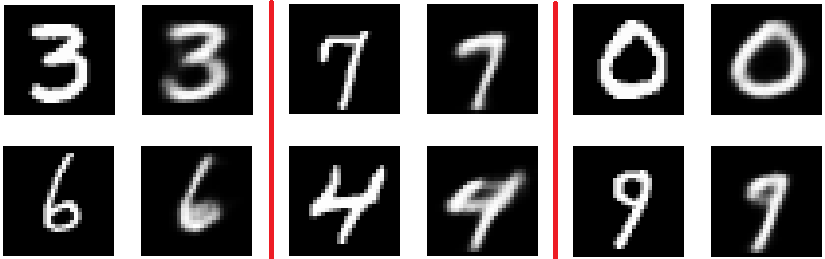
\includegraphics[width=0.35\textwidth]{figures/aae_sampling_real_reconstructed.png}
            \caption{Samples of autoencoder work. Left image is real, right is reconstructed.}
        \end{figure}
    \end{center}
    \subsection{Natalia's results}
    Training approach can be seen in git.

    The most enchanting thing here is evolution with epochs.
    The results for CIFAR are not good at all. Here the latent dimension is 8 the same as for MNIST.
    \begin{center}
        \begin{figure}[H]{\textwidth}
            \begin{subfigure}{0.5\textwidth}
                \centering
                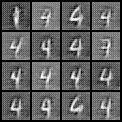
\includegraphics[width=0.35\linewidth]{figures/samples_67.jpg}
                \caption{MNIST, 67 epochs}
            \end{subfigure}
            \begin{subfigure}{0.5\textwidth}
                \centering
                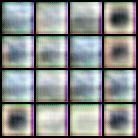
\includegraphics[width=0.35\linewidth]{figures/samples_55.jpg}
                \caption{CIFAR, 55 epochs}
            \end{subfigure}%
            \caption{Original paper algorithm results for the latest epochs}
        \end{figure}
    \end{center}
    \begin{center}
        \begin{figure}[H]
            \centering
            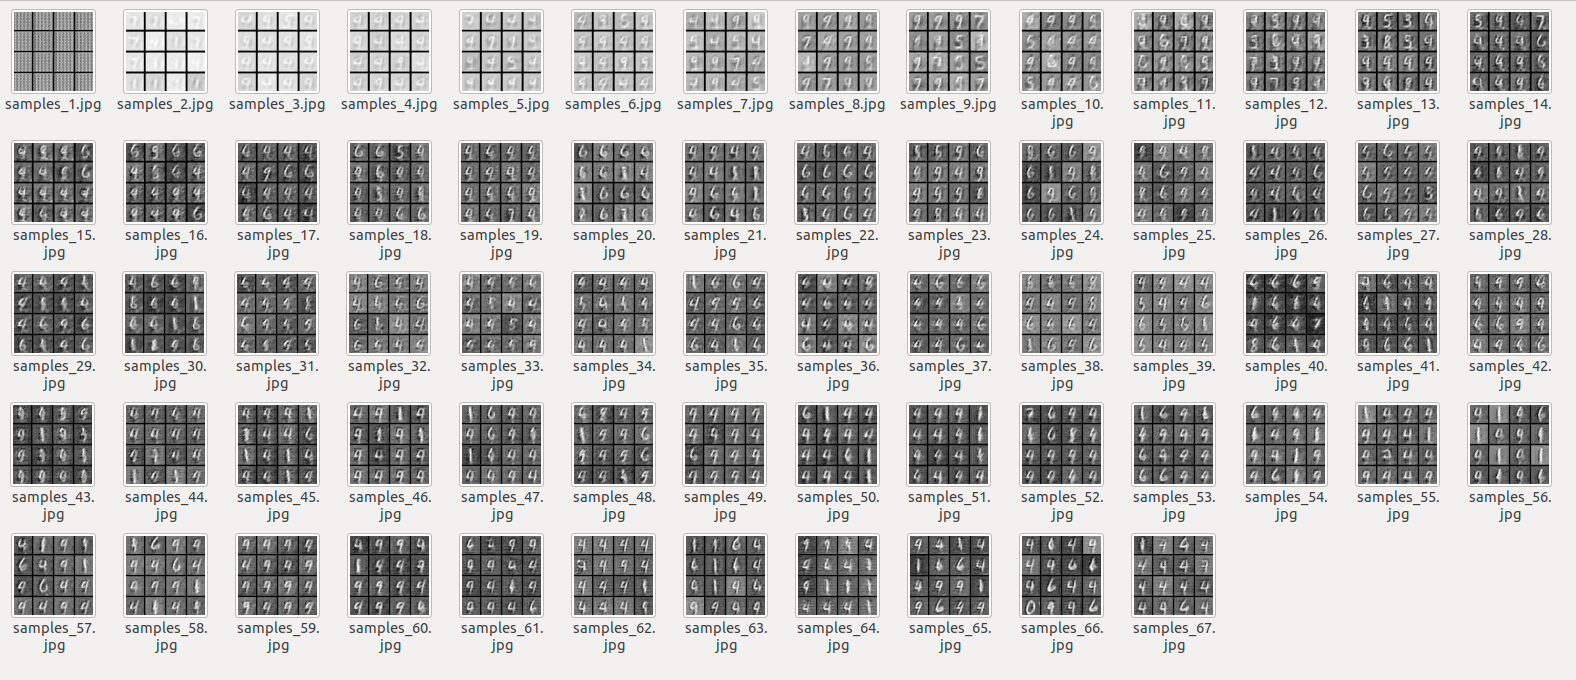
\includegraphics[width=0.6\textwidth]{figures/MNIST-original-evolution.png}
            \caption{Results evolution for original paper. MNIST}
        \end{figure}
    \end{center}
    \begin{center}
        \begin{figure}[H]
            \centering
            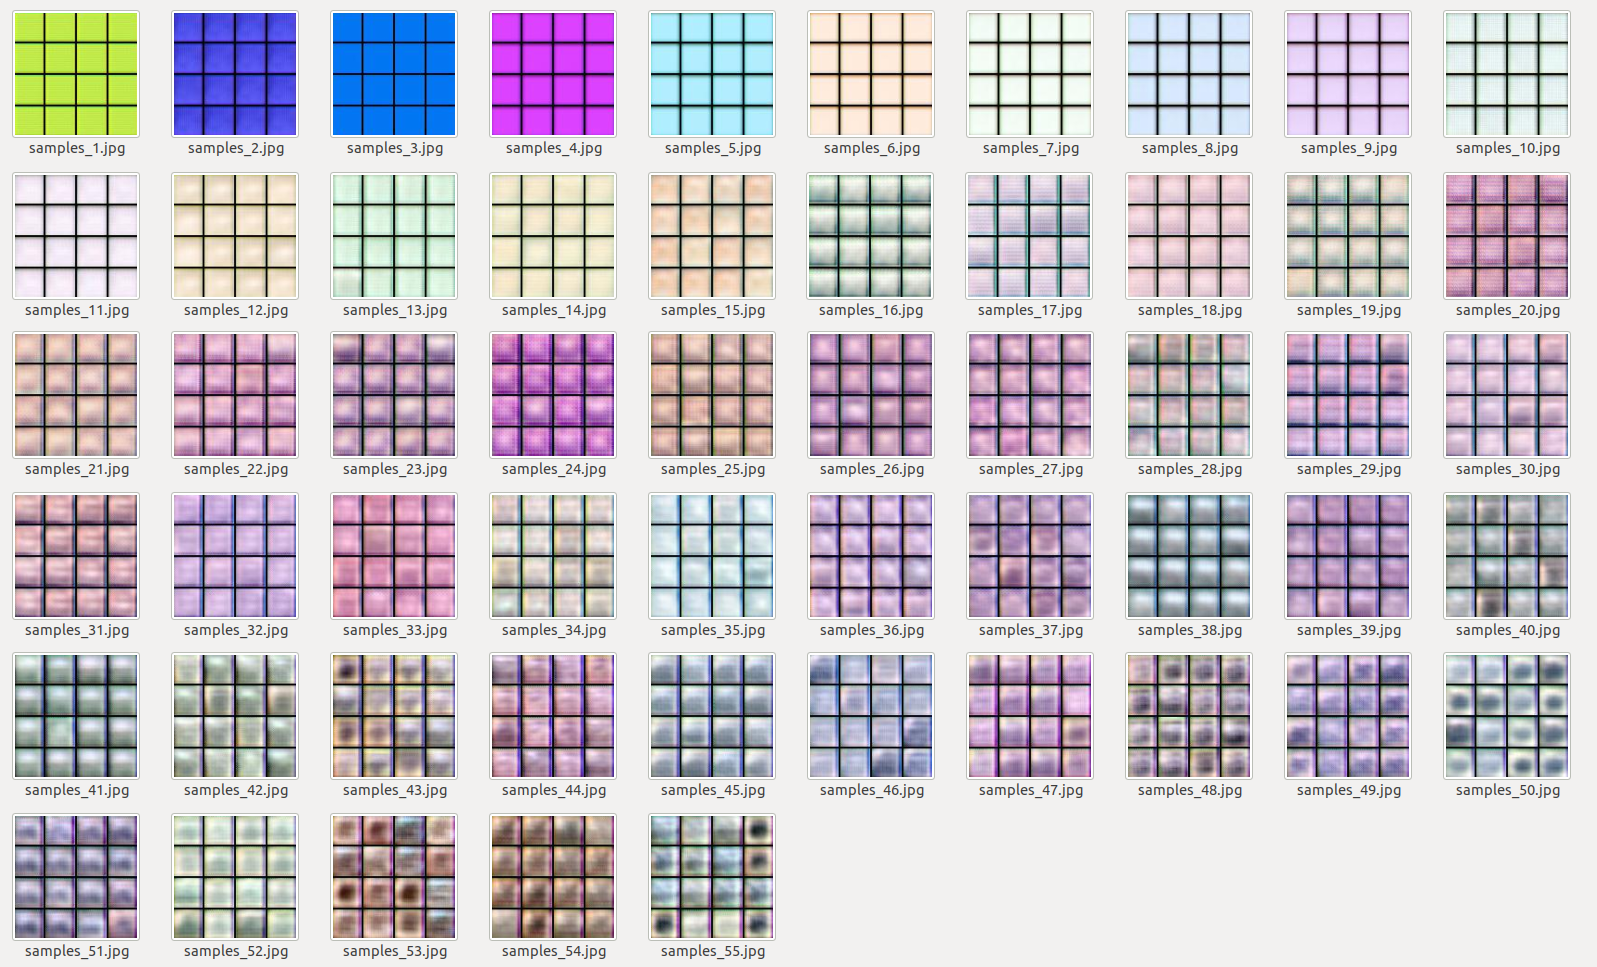
\includegraphics[width=0.5\textwidth]{figures/CIFAR-original-evolution.png}
            \caption{Results evolution for original paper. CIFAR}
        \end{figure}
    \end{center}


    \subsection{Results for additional algorithm}
    \begin{center}
        \begin{figure}[H]
            \centering
            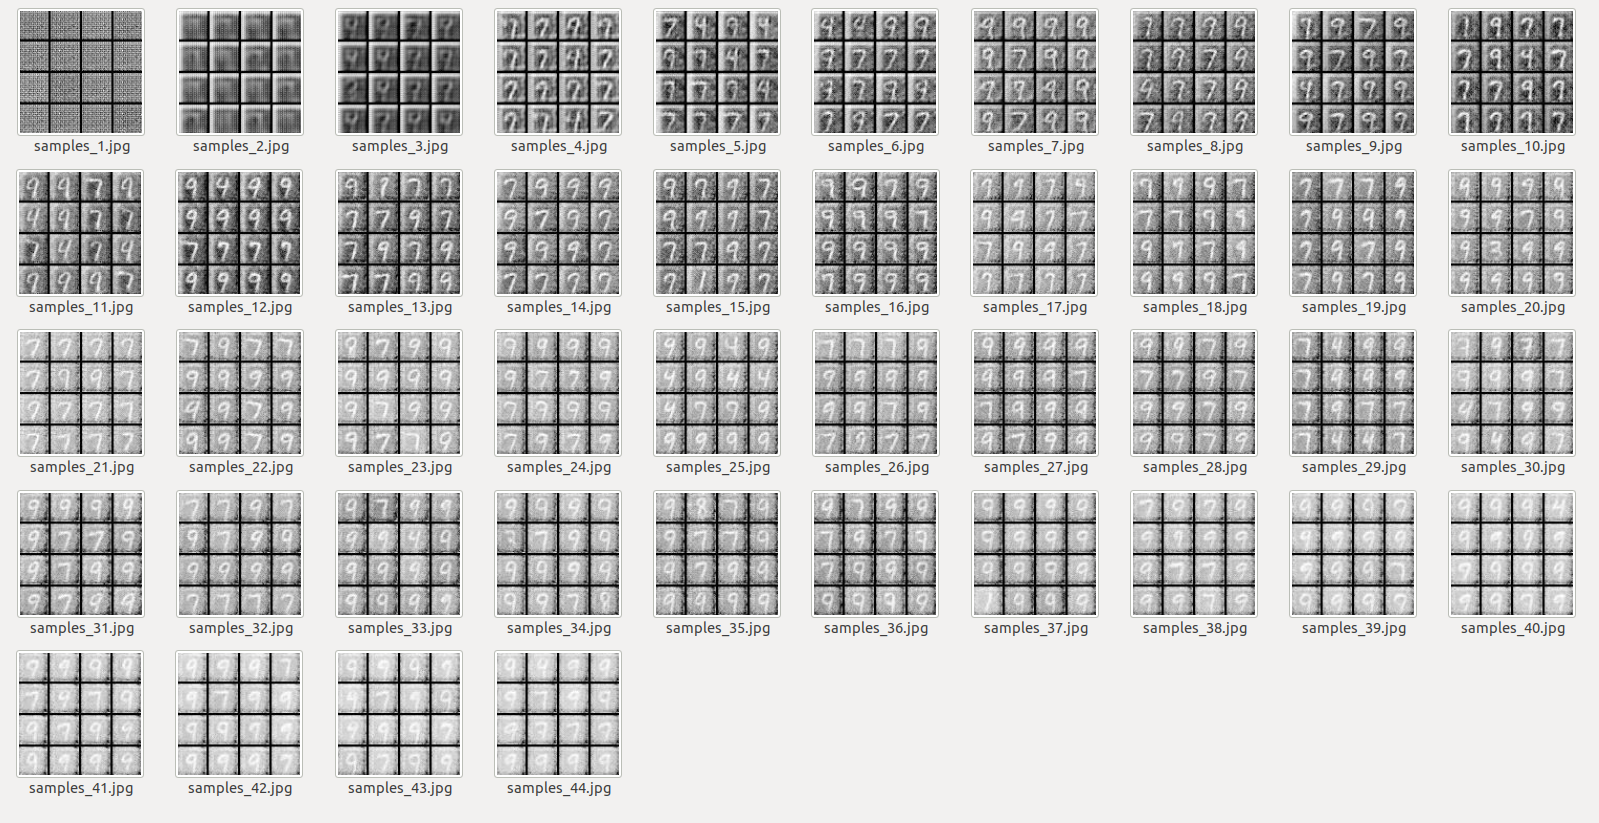
\includegraphics[width=0.6\textwidth]{figures/MNIST-additional-evolution.png}
            \caption{Results evolution for additional algorithm. MNIST}
        \end{figure}
    \end{center}

    \subsection{Conclusions}
    \begin{itemize}
        \item The adversarial training is difficult
        \item There are a lot of different schemes of generative models combining GAN and VAE
    \end{itemize}

    \subsection{Contributions}
    \begin{itemize}
        \item Belozerova Polina: reading papers, overview of mathematical model of VAE and GAN for structure prediction
        \item Safin Alexander: reading papers,
        implement the classical AAE,
        experiments for MNIST for classical AAE,
        MNIST and CIFAR for original paper approach,
        corresponding parts in the presentation and report
        \item Pavlovskaia Natalia: reading papers,
        implement the original paper,
        implement the additional algorithm,
        experiments for MNIST for both algorithms,
        experiments for CIFAR-10 for original paper,
        corresponding parts in the presentation and report
    \end{itemize}

    \bibliographystyle{unsrt}
    \bibliography{references}

\end{document}
